\documentclass[12pt]{article}

\usepackage{amsmath}
\usepackage{array}
\usepackage{caption}
\usepackage[top=1in, bottom=1in, left=0.75in, right=0.75in]{geometry}
\usepackage{graphicx}
\usepackage[colorlinks=true, allcolors=blue]{hyperref}
\usepackage[utf8]{inputenc}
\usepackage{multirow}
\usepackage{pdfpages}
\usepackage[section]{placeins}

\graphicspath{{figures/}}

\begin{document}

\begin{titlepage}
  \begin{center} \LARGE
    \vspace*{1.5in}

    ECE 272 Lab 3

    Fall 2018

    \vfill

    Combinational Logic (Seven-Segment Driver)

    Phi Luu

    \vfill

    October 24\textsuperscript{th}, 2018

    Grading TA: Edgar Perez

    Lab Partner: Benjamin Geyer

    \vspace{1.5in}
  \end{center}
\end{titlepage}

%%%%%%%%%%%%%%%%%%%%%%%%%%%%%%%%%%%%%%%%%%%%%%%%%%%%%%%%%%%%%%%%%%%%%%%%%%%%%%%%
% Introduction
%%%%%%%%%%%%%%%%%%%%%%%%%%%%%%%%%%%%%%%%%%%%%%%%%%%%%%%%%%%%%%%%%%%%%%%%%%%%%%%%
\section{Introduction}

Seven-segment displays are used in various electronic devices, such as microwave, digital clock, and video cassette players. They are one of the most popular choices to display numbers and most letters on digital devices due to their easy programming and user interfaces.

A seven-segment display has seven LEDs arranged in the shape of the digit 8. Each segment has its own signal name, and all segments connect to the decoder separately. There can be an additional LEDs which has a circle shape next to the digit, representing a decimal place. Figure~\ref{figure:1} shows what a seven-segment display looks like.

\begin{figure}[ht]
  \centering
  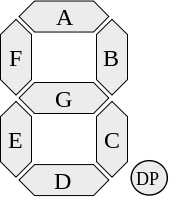
\includegraphics[width=0.25\textwidth]{seven_segment_display.png}
  \caption{The LED segments and their order in a seven-segment display\cite{WikimediaSevenSegment}}
  \label{figure:1}
\end{figure}

In this lab, I and Ben design a seven-segment display capable of displaying hexadecimal digits. We make a decoder that convert a 4-bit binary number into a single digit on the seven-segment display. The LED layout of each of the hexadecimal digits is as follows in Figure~\ref{figure:2}:

\begin{figure}[ht]
  \centering
  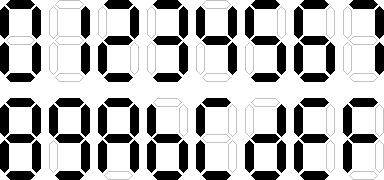
\includegraphics[width=0.5\textwidth]{seven_segment_hexadecimal.png}
  \caption{Seven-segment display showing hexadecimal digits \cite{EEStackExchangeSevenSegmentHex}}
  \label{figure:2}
\end{figure}

\newpage

%%%%%%%%%%%%%%%%%%%%%%%%%%%%%%%%%%%%%%%%%%%%%%%%%%%%%%%%%%%%%%%%%%%%%%%%%%%%%%%%
% Design
%%%%%%%%%%%%%%%%%%%%%%%%%%%%%%%%%%%%%%%%%%%%%%%%%%%%%%%%%%%%%%%%%%%%%%%%%%%%%%%%
\section{Design}

We use four switches to represent 4-bit binary numbers as inputs and a seven-segment display---or 7 LED segments---as outputs. To make outputs change accordingly (and correctly) to different values of the inputs, our objective is to use combinational logic to program a seven-segment display decoder on the FPGA. A visual representation of our objective is illustrated by the block diagram in Figure~\ref{figure:3}.

\begin{figure}[ht]
  \centering
  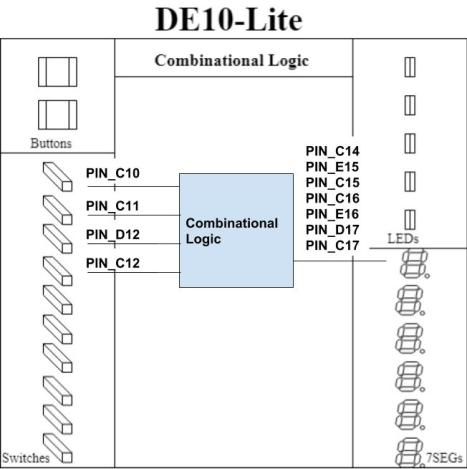
\includegraphics[width=0.5\textwidth]{lab3_block_diagram.png}
  \caption{Block diagram}
  \label{figure:3}
\end{figure}

Since the LED segments on the display are active-low---which means the pins will be active if low voltage is applied to it, the LED segment will turn on if the output signal is $0$ and turn off if the signal is $1$. Using the segment layout and digit syntax in Figures~\ref{figure:1} and~\ref{figure:2}, we construct the following truth table:

\newpage

\begin{table}[ht]
  \centering
  \begin{tabular}{ | c | c | c | c | c | c | c | c | c | }
  \hline \rule{0em}{1.15em}
  \textbf{\begin{tabular}[c]{@{}c@{}}Input\\ (Hexadecimal)\end{tabular}} & \textbf{\begin{tabular}[c]{@{}c@{}}Input\\ (4-bit Binary)\end{tabular}} & \textbf{Seg\textsubscript{A}} & \textbf{Seg\textsubscript{B}} & \textbf{Seg\textsubscript{C}} & \textbf{Seg\textsubscript{D}} & \textbf{Seg\textsubscript{E}} & \textbf{Seg\textsubscript{F}} & \textbf{Seg\textsubscript{G}} \\ \hline \rule{0em}{1.15em}
  0                                                                      & 0000                                                                    & 0                             & 0                             & 0                             & 0                             & 0                             & 0                             & 1                             \\ \hline \rule{0em}{1.15em}
  1                                                                      & 0001                                                                    & 1                             & 0                             & 0                             & 1                             & 1                             & 1                             & 1                             \\ \hline \rule{0em}{1.15em}
  2                                                                      & 0010                                                                    & 0                             & 0                             & 1                             & 0                             & 0                             & 1                             & 0                             \\ \hline \rule{0em}{1.15em}
  3                                                                      & 0011                                                                    & 0                             & 0                             & 0                             & 0                             & 1                             & 1                             & 0                             \\ \hline \rule{0em}{1.15em}
  4                                                                      & 0100                                                                    & 1                             & 0                             & 0                             & 1                             & 1                             & 0                             & 0                             \\ \hline \rule{0em}{1.15em}
  5                                                                      & 0101                                                                    & 0                             & 1                             & 0                             & 0                             & 1                             & 0                             & 0                             \\ \hline \rule{0em}{1.15em}
  6                                                                      & 0110                                                                    & 0                             & 1                             & 0                             & 0                             & 0                             & 0                             & 0                             \\ \hline \rule{0em}{1.15em}
  7                                                                      & 0111                                                                    & 0                             & 0                             & 0                             & 1                             & 1                             & 1                             & 1                             \\ \hline \rule{0em}{1.15em}
  8                                                                      & 1000                                                                    & 0                             & 0                             & 0                             & 0                             & 0                             & 0                             & 0                             \\ \hline \rule{0em}{1.15em}
  9                                                                      & 1001                                                                    & 0                             & 0                             & 0                             & 0                             & 1                             & 0                             & 0                             \\ \hline \rule{0em}{1.15em}
  a                                                                      & 1010                                                                    & 0                             & 0                             & 0                             & 1                             & 0                             & 0                             & 0                             \\ \hline \rule{0em}{1.15em}
  b                                                                      & 1011                                                                    & 1                             & 1                             & 0                             & 0                             & 0                             & 0                             & 0                             \\ \hline \rule{0em}{1.15em}
  c                                                                      & 1100                                                                    & 0                             & 1                             & 1                             & 0                             & 0                             & 0                             & 1                             \\ \hline \rule{0em}{1.15em}
  d                                                                      & 1101                                                                    & 1                             & 0                             & 0                             & 0                             & 0                             & 1                             & 0                             \\ \hline \rule{0em}{1.15em}
  e                                                                      & 1110                                                                    & 0                             & 1                             & 1                             & 0                             & 0                             & 0                             & 0                             \\ \hline \rule{0em}{1.15em}
  f                                                                      & 1111                                                                    & 0                             & 1                             & 1                             & 1                             & 0                             & 0                             & 0                             \\ \hline
  \end{tabular}
  \caption{Conversion table between hexadecimal, 4-bit binary, and seven-segment decoder}
  \label{table:1}
\end{table}

Using Table~\ref{table:1}, the digit $0$ in hexadecimal system is equivalent to $0000$ in binary system. Segments A through F in the decoder are lit up, and segment G will be turned off---this is exactly what Figure~\ref{figure:2} illustrates. The remaining rows of the table are interpreted in the same way.

From Table~\ref{table:1}, we can write a sum-of-product form for each of the segments using their minterms. \textbf{Note that even though the segments are active-low, the Boolean equations still use rows with output 1 (since they are the minterms, and minterms always use 1).}

We want to simplify the Boolean equation of each of the segments as much as possible so that we can use minimal hardware when building the circuit of the decoder. Therefore, we use Karnaugh maps to simplify the Boolean equations of the segments, as demonstrated on the next page.

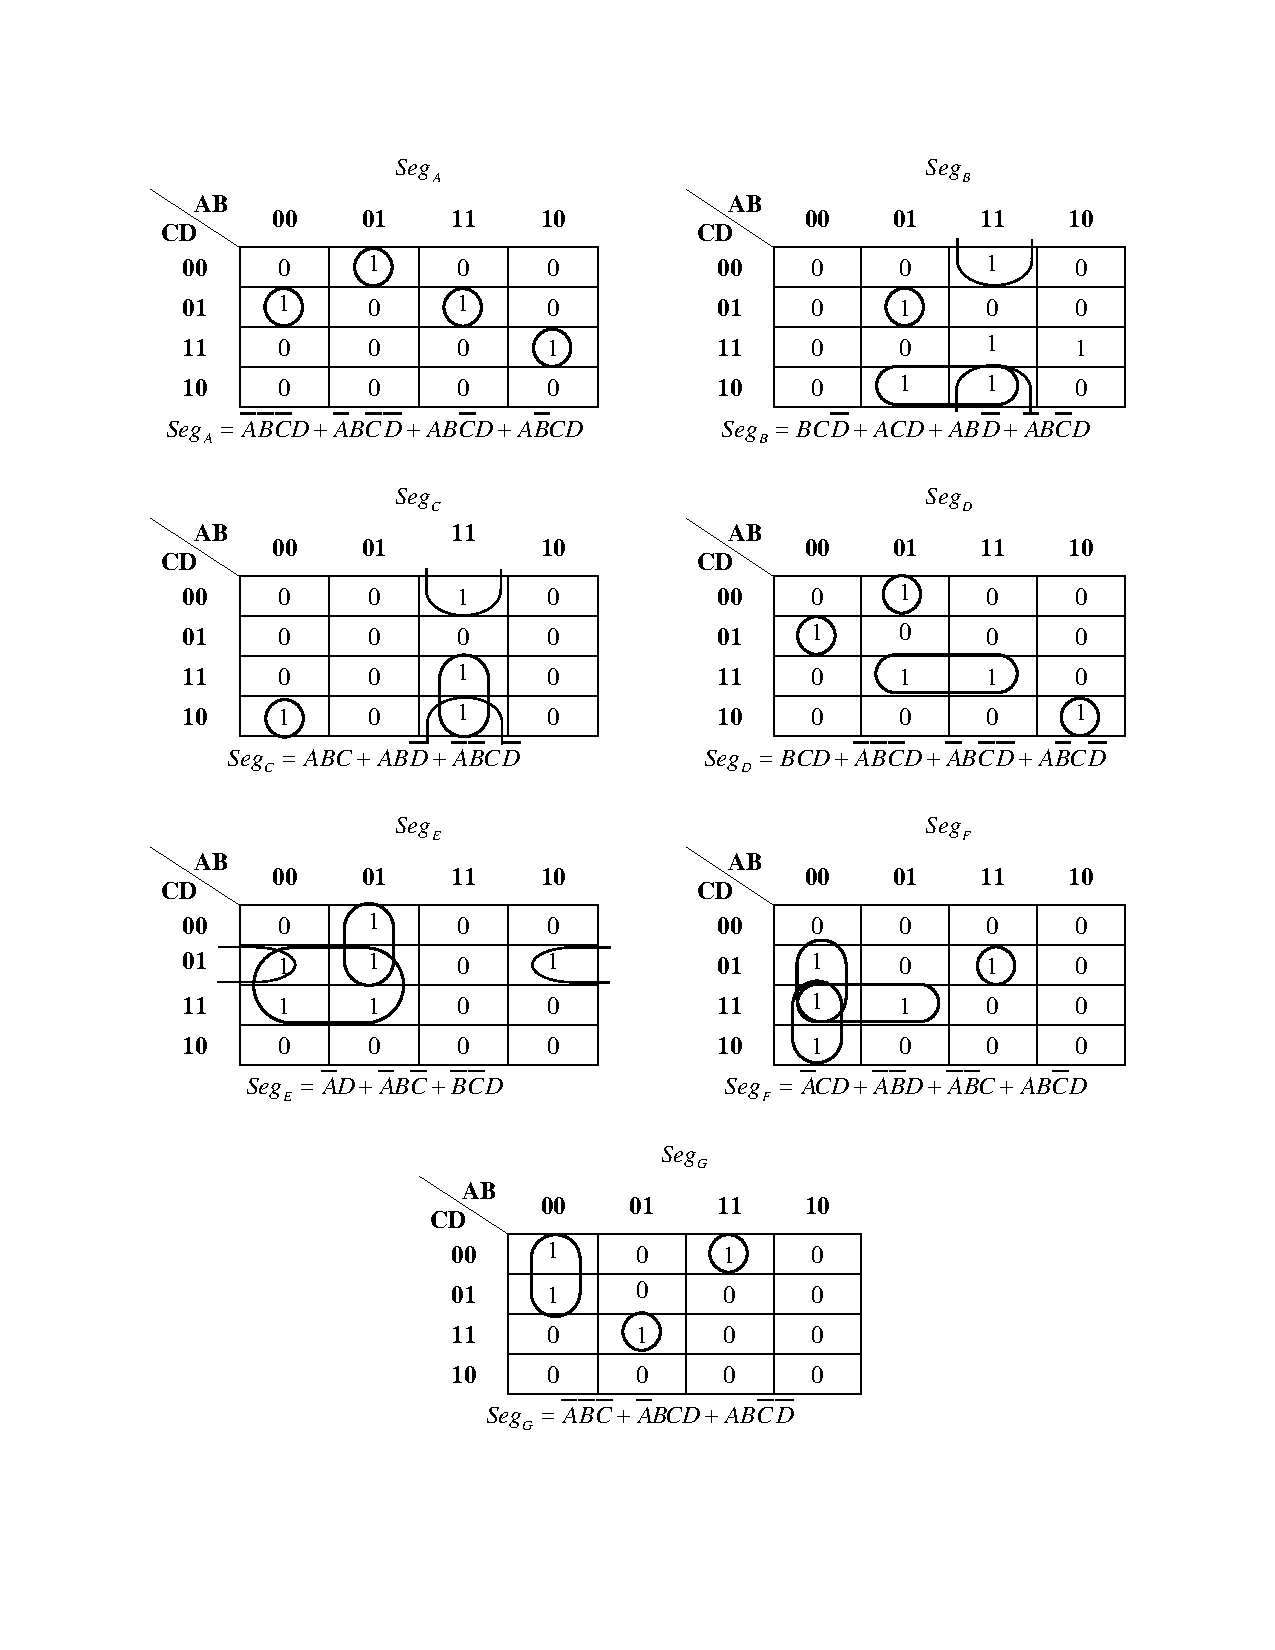
\includepdf[page=-]{lab3_karnaugh_maps}

There are a few Boolean terms that appears in more than one Boolean equations, such as $\bar{A}B\bar{C}\bar{D}$ and $\bar{A}\bar{B}\bar{C}D$ in segments A and D. Hence, the logic gates can be reused, which further simplifies the hardware needed to build the circuit. A schematic of the circuit is as in Figure~\ref{figure:4} below.

\begin{figure}[ht]
  \centering
  \includegraphics[width=\textwidth]{lab3_schematic.png}
  \caption{A schematic for the seven-segment display decoder. Due to the large difference between the size of the schematic and the available space, an image with higher resolution has been uploaded \href{https://i.imgur.com/jaLoZg9.jpg}{here}.}
  \label{figure:4}
\end{figure}

The schematic of the decoder is indeed complicated, yet it can be easier read when divided into smaller groups. A simpler way to read the schematic is that there are seven group of combinational logic gates and 8 input buses (4 bits of input and their inversions).

%%%%%%%%%%%%%%%%%%%%%%%%%%%%%%%%%%%%%%%%%%%%%%%%%%%%%%%%%%%%%%%%%%%%%%%%%%%%%%%%
% Results
%%%%%%%%%%%%%%%%%%%%%%%%%%%%%%%%%%%%%%%%%%%%%%%%%%%%%%%%%%%%%%%%%%%%%%%%%%%%%%%%
\section{Results}

We test the schematic on the simulator. For each 10-ns time interval, we try a hexadecimal digit on the inputs: 0 for 0--10.0 ns, 1 for 10.0 ns--20.0 ns, 2 for 20.0 ns--30.0 ns, and so on. We obtain the following results:

\begin{figure}[ht]
  \centering
  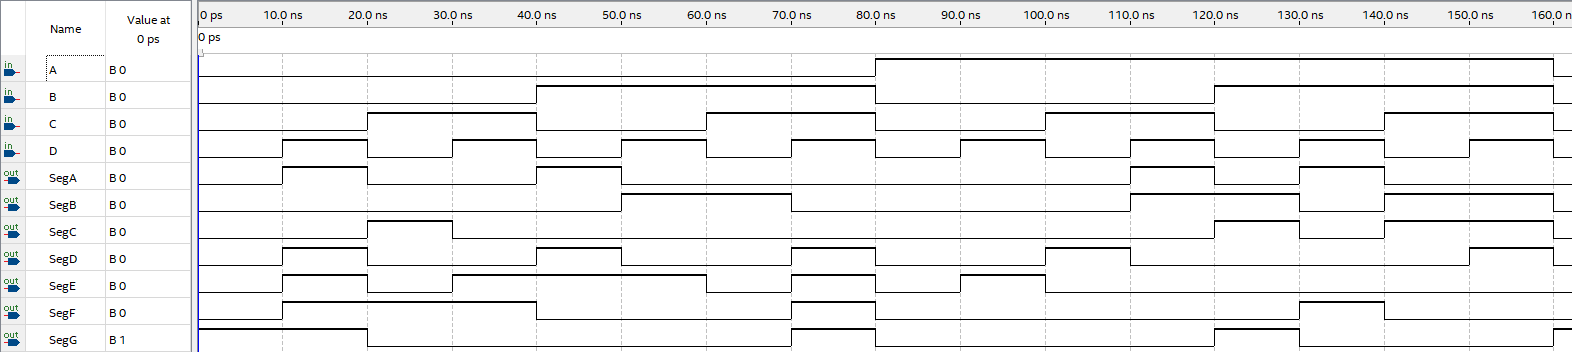
\includegraphics[width=\textwidth]{lab3_simulation.png}
  \caption{Simulation waveform of the program with each 10-nanosecond interval representing a hexadecimal digit}
  \label{figure:5}
\end{figure}

After running the simulation, we observe that when the input is $0$, the output signal (segments A through G) is $0000001$; when the input is $1$, the output signal is $1001111$; and so on. The simulation outputs are the same as expected the outputs in Table~\ref{table:1}.

The seven-segment display behaves as expected when we upload the program to the FPGA. Therefore, the seven-segment display decoder is successfully implemented.

%%%%%%%%%%%%%%%%%%%%%%%%%%%%%%%%%%%%%%%%%%%%%%%%%%%%%%%%%%%%%%%%%%%%%%%%%%%%%%%%
% Experiment Notes
%%%%%%%%%%%%%%%%%%%%%%%%%%%%%%%%%%%%%%%%%%%%%%%%%%%%%%%%%%%%%%%%%%%%%%%%%%%%%%%%
\section{Experiment Notes}

%%%%%%%%%%%%%%%%%%%%%%%%%%%%%%%%%%%%%%%%
% Reflection
%%%%%%%%%%%%%%%%%%%%%%%%%%%%%%%%%%%%%%%%
\subsection*{Reflection}

This lab was quite challenging when we approached it without the idea of logic simplification in mind. In fact, we couldn't figure out which direction to take to implement the decoder. However, when we took a step back and analyzed the problem carefully, we realized that this problem was just another truth-table-to-Boolean-equation simplification type of problems. Things became much easier after we constructed the truth table and Karnaugh maps. The rest of the problem was an easy technical process.

%%%%%%%%%%%%%%%%%%%%%%%%%%%%%%%%%%%%%%%%
% Study Questions
%%%%%%%%%%%%%%%%%%%%%%%%%%%%%%%%%%%%%%%%
\subsection*{Study Questions}

\begin{enumerate}
  \item When is a simulation necessary? Was it useful for this section?

  When testing a program before deploying it into a real system, simulation is very important. A program without thorough testing could cause various problems, including breaking the system and/or causing the hardware to malfunction. Simulation process was quite useful for this section because we can anticipate what will happen when the program is uploaded to the real FPGA by analyzing the simulation waveform. We can fix program bugs and flaws before they even get into the FPGA. We believe that a program should go through a simulation process before going into a real system.
\end{enumerate}

%%%%%%%%%%%%%%%%%%%%%%%%%%%%%%%%%%%%%%%%%%%%%%%%%%%%%%%%%%%%%%%%%%%%%%%%%%%%%%%%
% Appendix
%%%%%%%%%%%%%%%%%%%%%%%%%%%%%%%%%%%%%%%%%%%%%%%%%%%%%%%%%%%%%%%%%%%%%%%%%%%%%%%%
\section*{Appendix}

No appendix is available in this lab.

%%%%%%%%%%%%%%%%%%%%%%%%%%%%%%%%%%%%%%%%%%%%%%%%%%%%%%%%%%%%%%%%%%%%%%%%%%%%%%%%
% Bibliography
%%%%%%%%%%%%%%%%%%%%%%%%%%%%%%%%%%%%%%%%%%%%%%%%%%%%%%%%%%%%%%%%%%%%%%%%%%%%%%%%
\bibliographystyle{ieeetr}
\bibliography{references}

\end{document}
